\section{Arquitectura técnica}\label{sec:arquitectura}

\subsection{Vista de software}

El sistema se compone de un frontend estático y dos servicios de backend que solo se comunican por
HTTP (Fig.~\ref{fig:software}):

\begin{itemize}
  \item \textbf{Frontend} (Next.js~16 exportado como sitio estático, React~19, Tailwind~v4): el
        planificador con el mapa (MapLibre sobre OpenFreeMap), la lista de viajes y la consola de
        administración. Interfaz bilingüe (español e inglés).
  \item \textbf{\code{core\_api}} (FastAPI): usuarios, viajes, lista de acceso y cuotas. Guarda sus
        datos en una tabla de DynamoDB con diseño de tabla única; \code{ai\_api} usa
        una segunda tabla, propia, para trazas y contadores de tokens.
  \item \textbf{\code{ai\_api}} (FastAPI): el planificador y su agente, la recuperación sobre la
        base vectorial, el detalle de tarjetas y la lectura de trazas para administración.
  \item \textbf{\code{travel\_common}}: núcleo compartido: identidad \code{Principal}, errores de
        dominio, verificación de tokens JWT (\emph{JSON Web Token}) y factoría de aplicaciones.
\end{itemize}

Separar la IA del núcleo transaccional permite que cada servicio escale, falle y se
despliegue por separado: un pico de uso del planificador no degrada el guardado de viajes, y el
servicio de IA puede cambiar de proveedor de modelos sin tocar los datos de usuario. Ninguno
importa código del otro, regla que se comprueba en cada revisión. Internamente ambos siguen una
arquitectura hexagonal: casos de uso que dependen de \emph{puertos} (\code{LLMProvider},
\code{Retriever}, \code{InputGuard}) con adaptadores intercambiables (Bedrock o NVIDIA; S3 Vectors
o un recuperador por palabras clave para pruebas), como muestra la Fig.~\ref{fig:software}.

\begin{figure}[t]
\centering
\resizebox{\columnwidth}{!}{\begin{tikzpicture}[x=1cm,y=1cm,
  lbl/.style={font=\fontsize{6}{7}\selectfont,color=kgray,align=center},
  p/.style={box,font=\scriptsize,text width=1.85cm,minimum height=0.5cm,inner sep=2pt},
  ad/.style={data,font=\scriptsize,text width=1.85cm,minimum height=0.5cm,inner sep=2pt},
  aa/.style={ai,font=\scriptsize,text width=1.85cm,minimum height=0.5cm,inner sep=2pt}]
\node[ext,font=\scriptsize,text width=8.1cm,minimum height=0.7cm] (fe) at (4.2,3.45) {\textbf{Navegador}: planificador con mapa, viajes y administración; guarda el estado del turno};
% core_api
\node[p,text width=2.5cm] (uc) at (1.45,2.2) {Casos de uso: usuarios, viajes, acceso};
\node[p,text width=2.5cm] (rp) at (1.45,1.35) {Puerto: repositorio};
\node[ad,text width=2.5cm] (ddb) at (1.45,0.5) {DynamoDB};
\draw[arr] (uc) -- (rp); \draw[arr] (rp) -- (ddb);
% ai_api
\node[aa,text width=4.1cm] (pt) at (6.3,2.2) {\code{PlanTrip}: pasos deterministas + agente Kiri};
\node[p] (llm) at (5.25,1.35) {\code{LLMProvider}};
\node[p] (ret) at (7.35,1.35) {\code{Retriever}};
\node[aa] (llma) at (5.25,0.5) {Bedrock | NVIDIA};
\node[ad] (reta) at (7.35,0.5) {S3 Vectors | léxico};
\node[p] (grd) at (5.25,-0.3) {\code{InputGuard}: \emph{Guardrail}};
\node[p] (trc) at (7.35,-0.3) {\code{Tracer}: DynamoDB};
\draw[arr] (pt.south -| llm) -- (llm); \draw[arr] (pt.south -| ret) -- (ret);
\draw[arr] (llm) -- (llma); \draw[arr] (ret) -- (reta);
\begin{scope}[on background layer]
\node[draw=kblue,rounded corners=3pt,fill=blue!2,fit=(uc)(rp)(ddb),inner sep=5pt,inner ysep=9pt,yshift=3pt] (corebox) {};
\node[draw=kpurple,rounded corners=3pt,fill=violet!2,fit=(pt)(llm)(ret)(llma)(reta)(grd)(trc),inner sep=5pt,inner ysep=9pt,yshift=3pt] (aibox) {};
\end{scope}
\node[font=\scriptsize\bfseries,color=kblue,anchor=north] at (corebox.north) {core\_api};
\node[font=\scriptsize\bfseries,color=kpurple,anchor=north] at (aibox.north) {ai\_api};
\draw[arr] (fe.south -| corebox.north) -- node[lbl,right]{REST} (corebox.north);
\draw[arr] (fe.south -| aibox.north) -- node[lbl,right]{SSE} (aibox.north);
\draw[arr] (aibox.west |- rp) -- node[lbl,above]{HTTP} node[lbl,below]{acceso} (corebox.east |- rp);
% común y datos
\node[box,font=\scriptsize,text width=8.1cm,minimum height=0.45cm] (common) at (4.2,-1.25) {\textbf{travel\_common}: identidad, errores de dominio, verificación de tokens, logs de acceso};
\draw[darr] (common.north -| corebox.south) -- (corebox.south);
\draw[darr] (common.north -| aibox.south) -- (aibox.south);
\node[data,font=\scriptsize,text width=3.1cm,minimum height=0.6cm] (corpus) at (1.8,-2.15) {\textbf{city\_corpus} (sin conexión): fuentes abiertas $\rightarrow$ JSONL};
\node[data,font=\scriptsize,text width=3.1cm,minimum height=0.6cm] (idx) at (6.3,-2.15) {\textbf{indexador}: Titan V2 $\rightarrow$ S3 Vectors};
\draw[arr] (corpus) -- node[lbl,above]{Git} (idx);
\end{tikzpicture}
}
\caption{Vista de software: dos servicios hexagonales que solo se comunican por HTTP, un núcleo común y el proceso de datos fuera de línea (\emph{offline}) que alimenta la base vectorial. Cada puerto tiene adaptadores intercambiables (producción | desarrollo y pruebas).}\label{fig:software}
\end{figure}

El planificador \textbf{no guarda estado}: el navegador guarda el resumen del viaje, el itinerario
(como identificadores de tarjeta) y la conversación, y los reenvía en cada turno. El servidor
nunca confía en el contenido de una tarjeta que llega del cliente: la reconstruye desde la base
vectorial por su identificador. Así, cualquier instancia del servicio (en producción, una función
Lambda; §\ref{sec:coste}) puede atender cualquier turno sin almacén de sesiones.

\begin{figure*}[tp]
\centering
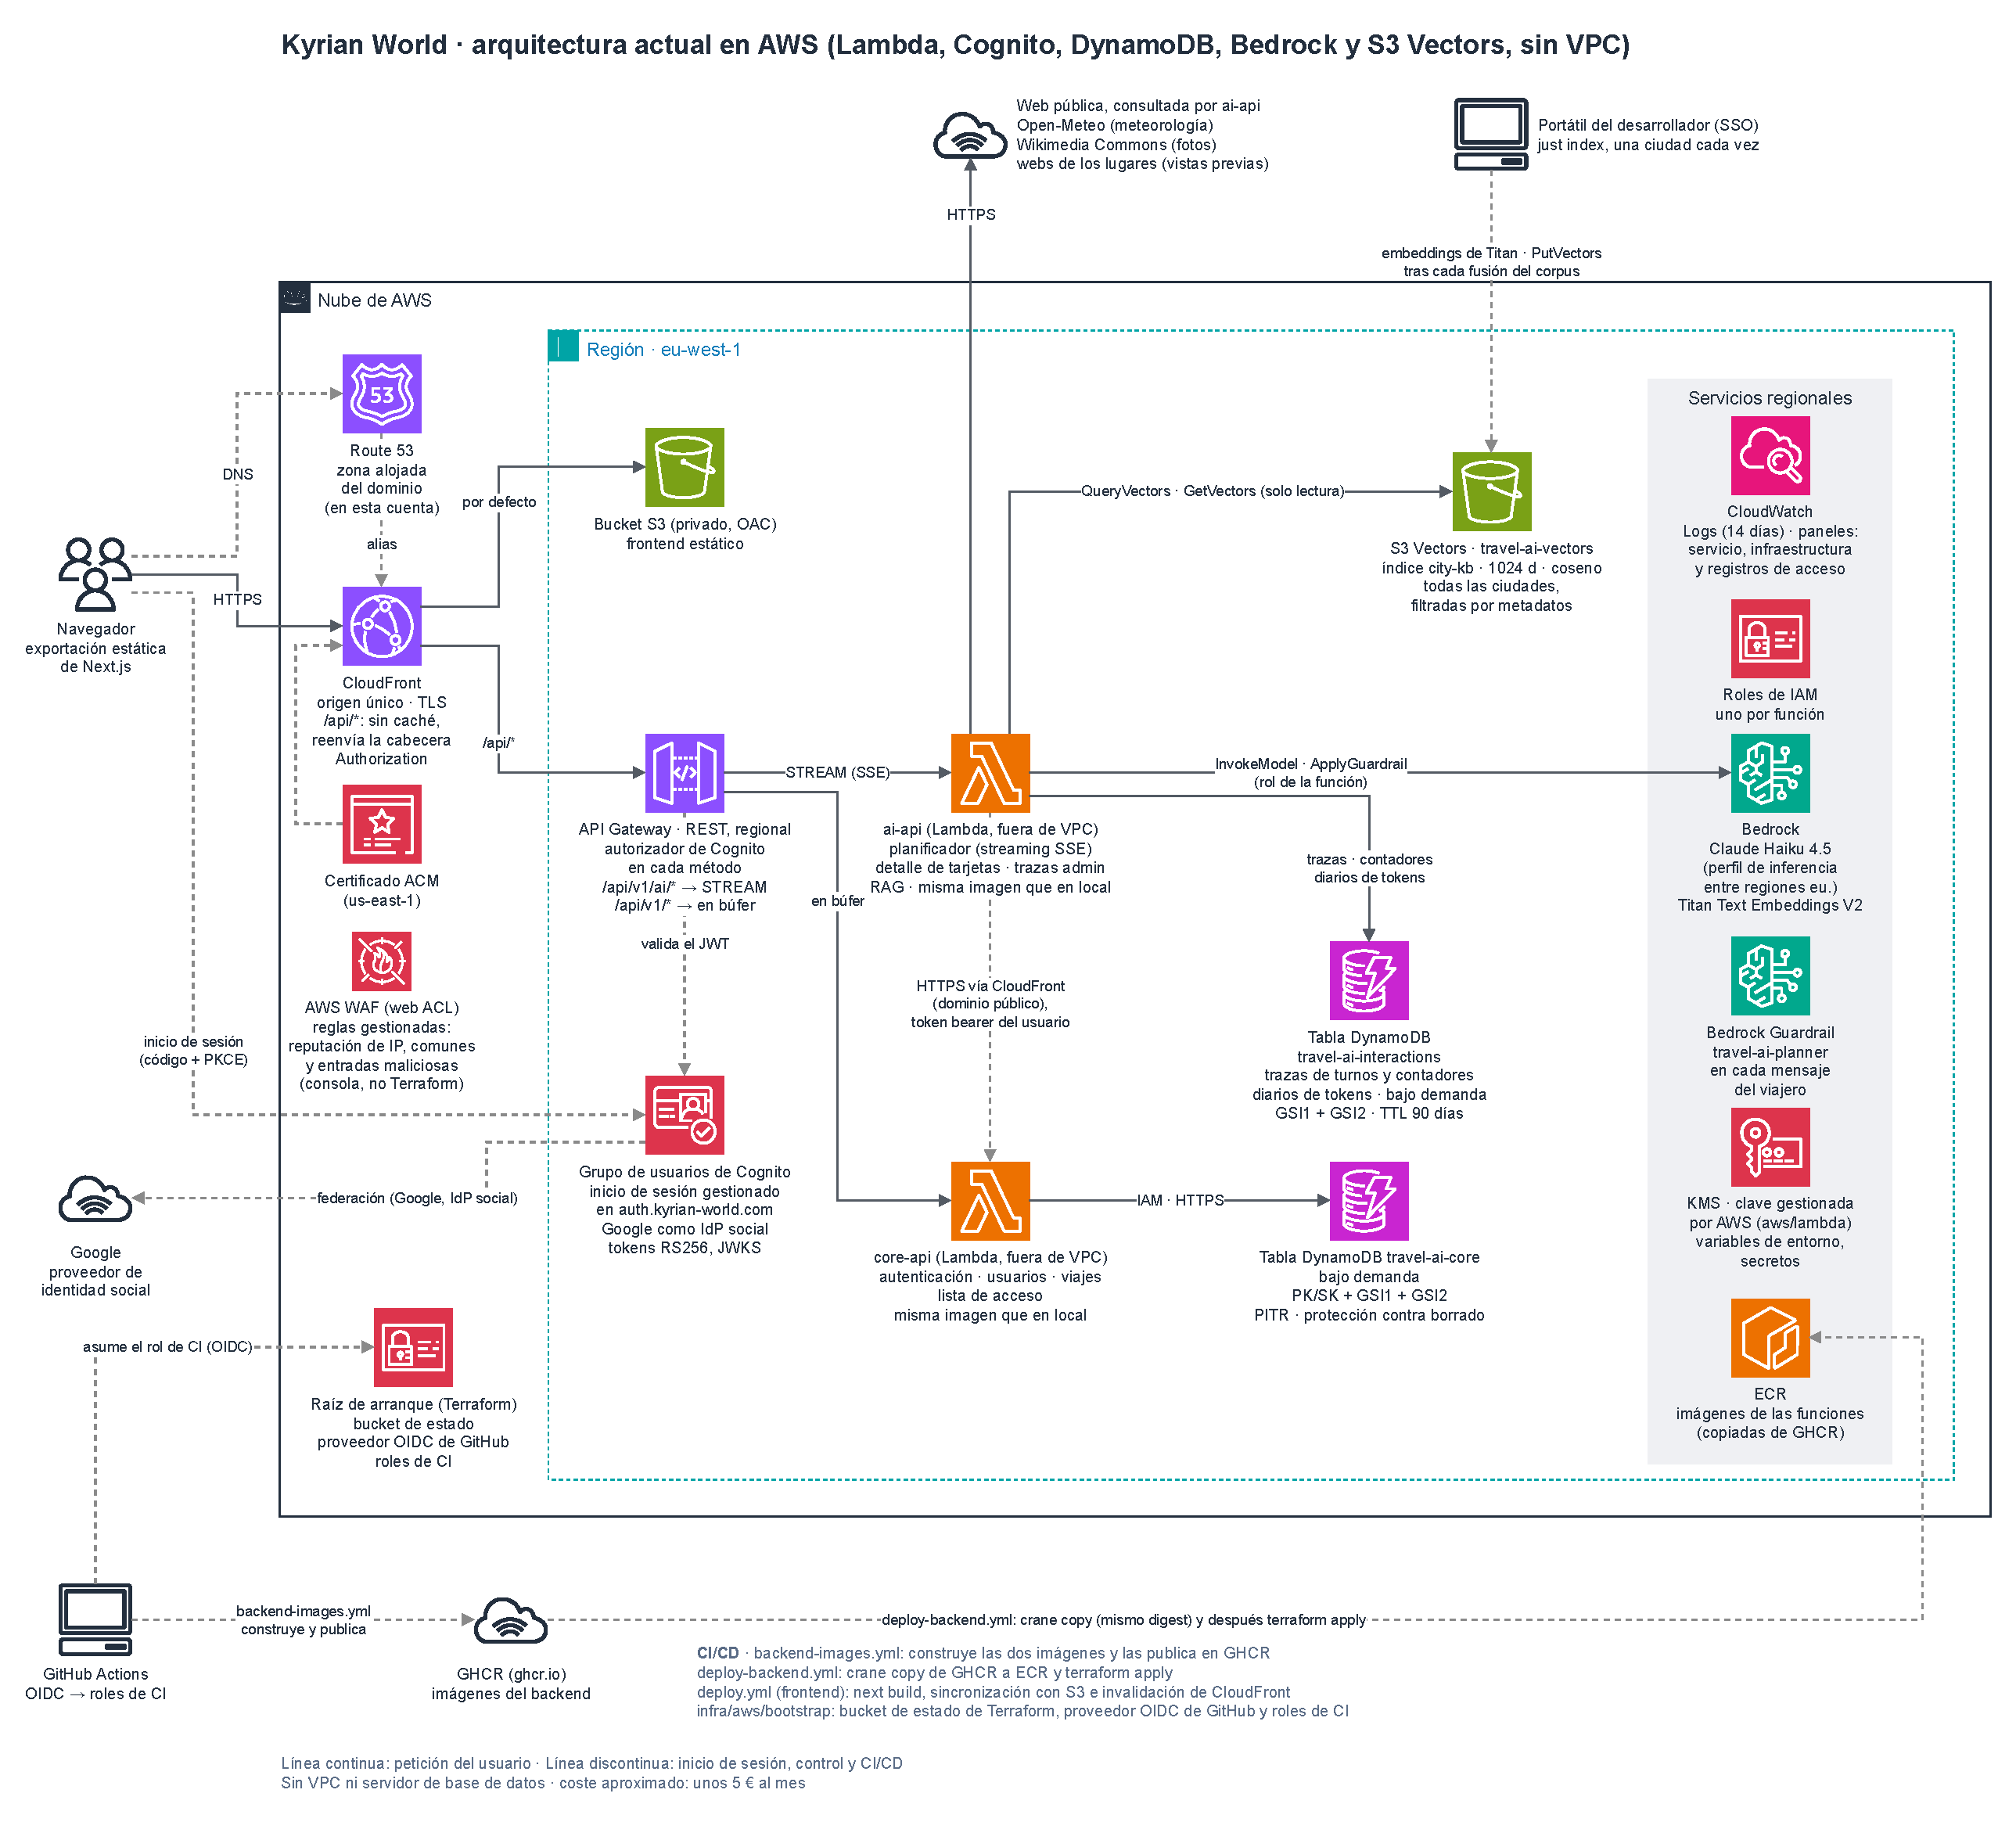
\includegraphics[width=\textwidth]{figs/aws-actual.pdf}
\caption{Arquitectura desplegada en AWS (\code{infra/aws}). Todo es gestionado y de pago por uso: no hay máquinas, VPC, NAT ni balanceadores. Comparte disposición con la arquitectura objetivo (Fig.~\ref{fig:objetivo}) para facilitar la comparación.}\label{fig:aws}
\end{figure*}

\subsection{Decisiones de arquitectura}\label{sec:decisiones}

La Tabla~\ref{tab:decisiones} resume las decisiones con más impacto. Esas y el resto, 36 en total,
están documentadas en el repositorio con las alternativas descartadas y el criterio empleado.

\begin{table}[t]
\centering\scriptsize
\caption{Decisiones principales (alternativa descartada y motivo).}\label{tab:decisiones}
\begin{tabularx}{\columnwidth}{@{}L{1.75cm}L{1.9cm}Y@{}}
\toprule
\textbf{Decisión} & \textbf{Descartado} & \textbf{Motivo} \\
\midrule
Lambda + API Gateway REST & ECS Fargate + NLB + RDS & Coste en reposo diez veces menor (Tabla~\ref{tab:coste}); escala a cero; la API REST admite \emph{streaming} de hasta 15\,min (la HTTP API lo corta a los 30\,s) \\
S3 Vectors & Qdrant en Lambda, pgvector, Qdrant Cloud & Igual calidad medida, coste de céntimos y sin servidores que operar (§\ref{sec:spike}) \\
DynamoDB tabla única & RDS PostgreSQL & Sin instancia en reposo; el agregado «viaje» se guarda en un único ítem \\
SSE tipado sin estado & WebSocket, sesión en servidor & Compatible con Lambda; el cliente aplica operaciones tipadas \\
Agente en proceso & Bedrock Agents, una Lambda por herramienta & Mantiene el contrato de eventos tipados y la latencia \\
Salidas estructuradas nativas & JSON pedido en el \emph{prompt} & El proveedor garantiza el esquema; menos reparaciones \\
Cognito + Google & JWT propio & Sin contraseñas que custodiar; 10.000 usuarios activos gratis \\
\bottomrule
\end{tabularx}
\end{table}

\subsection{Nube 100\,\% \emph{serverless}: siempre en línea al menor coste}\label{sec:coste}

La arquitectura actual es la tercera iteración. La primera, un prototipo con contenedores en ECS y
Cloud Run, sirvió para explorar; la segunda, diseñada pero no desplegada (ECS Fargate y RDS),
costaba unos 55\,€/mes sin contar aún la salida a Internet (NAT), frente a un presupuesto de 60\,€
para dos meses. Se migró a una arquitectura (Fig.~\ref{fig:aws}) en la que \textbf{nada se paga
en reposo y todo es un servicio gestionado y redundante por defecto}. Recorriendo la figura de
izquierda a derecha:

\begin{itemize}
  \item \textbf{Borde}: CloudFront sirve el sitio estático desde S3 y enruta \code{/api/*} a API
        Gateway desde el mismo origen, de modo que no hace falta configurar CORS (intercambio
        de recursos entre orígenes). Las respuestas de la API no se cachean ni se
        comprimen para que el \emph{streaming} llegue intacto.
  \item \textbf{Cómputo}: dos funciones de AWS Lambda (cómputo bajo demanda, sin servidores)
        empaquetadas como imagen de contenedor. FastAPI corre sin cambios gracias a
        AWS Lambda Web Adapter~\cite{awslwa}, una extensión que traduce cada invocación en una
        petición HTTP local y que fuera de Lambda no hace nada: la misma imagen funciona en Docker
        Compose y en Lambda. La función de IA transmite la respuesta en \emph{streaming} durante un máximo de
        15 minutos.
  \item \textbf{Datos}: DynamoDB bajo demanda (con recuperación a un momento dado, PITR, en la tabla
        principal) y S3 Vectors~\cite{aws2025s3vectors}: vectores en S3, cobro por consulta, sin clúster.
  \item \textbf{IA}: Bedrock factura por token, y Bedrock Guardrails, por unidad de texto evaluada.
\end{itemize}

\begin{table}[t]
\centering\scriptsize
\caption{Coste mensual estimado con precios de lista en eu-west-1 y tráfico de demostración (estimación documentada en el repositorio).}\label{tab:coste}
\begin{tabularx}{\columnwidth}{@{}Yr@{}}
\toprule
\textbf{Servicio} & \textbf{€/mes} \\
\midrule
Lambda (2 funciones; capa gratuita permanente) & 0 \\
API Gateway REST (3,50\,\$ por millón de peticiones) & $<$1 \\
CloudFront + S3 + Route 53 & $\approx$1 \\
Cognito (gratis hasta 10.000 usuarios activos) & 0 \\
DynamoDB bajo demanda (2 tablas) + PITR & $<$1 \\
ECR, CloudWatch Logs & $\approx$1 \\
Bedrock (uso de demostración) y S3 Vectors & 1--3 \\
\midrule
\textbf{Total de la plataforma} & \textbf{$\approx$5} \\
WAF de CloudFront (3 grupos de reglas gestionadas; opcional; $\approx$8\,\$) & $\approx$7 \\
\bottomrule
\end{tabularx}
\end{table}

«Siempre en línea» no depende de mantener instancias encendidas: CloudFront, Lambda, DynamoDB y
S3 son multizona por diseño y escalan con la demanda. Las dos contrapartidas habituales de
Lambda están acotadas en el diseño. La primera son los arranques en frío: afectan a una minoría de
invocaciones (en producción, el 10,7\,\% en \code{ai\_api} y el 6,4\,\% en \code{core\_api}, con
unos 2,4--2,5\,s de inicialización mediana), y en cuanto la función arranca el navegador recibe eventos
de progreso, de modo que la espera se percibe como parte del turno; la arquitectura objetivo los
elimina (§\ref{sec:prod}). La segunda es que Lambda no ejecuta tareas en segundo plano tras
responder; por eso las trazas y los contadores se escriben \emph{antes} de cerrar el flujo, lo que
además garantiza que ningún turno quede sin trazar. El cortafuegos de aplicaciones web (WAF) es un
coste aparte y opcional (Tabla~\ref{tab:coste}): protege el borde con reglas gestionadas y más que
duplica la factura en reposo, por lo que se trata como una decisión de presupuesto independiente.

\begin{figure*}[!t]
\centering
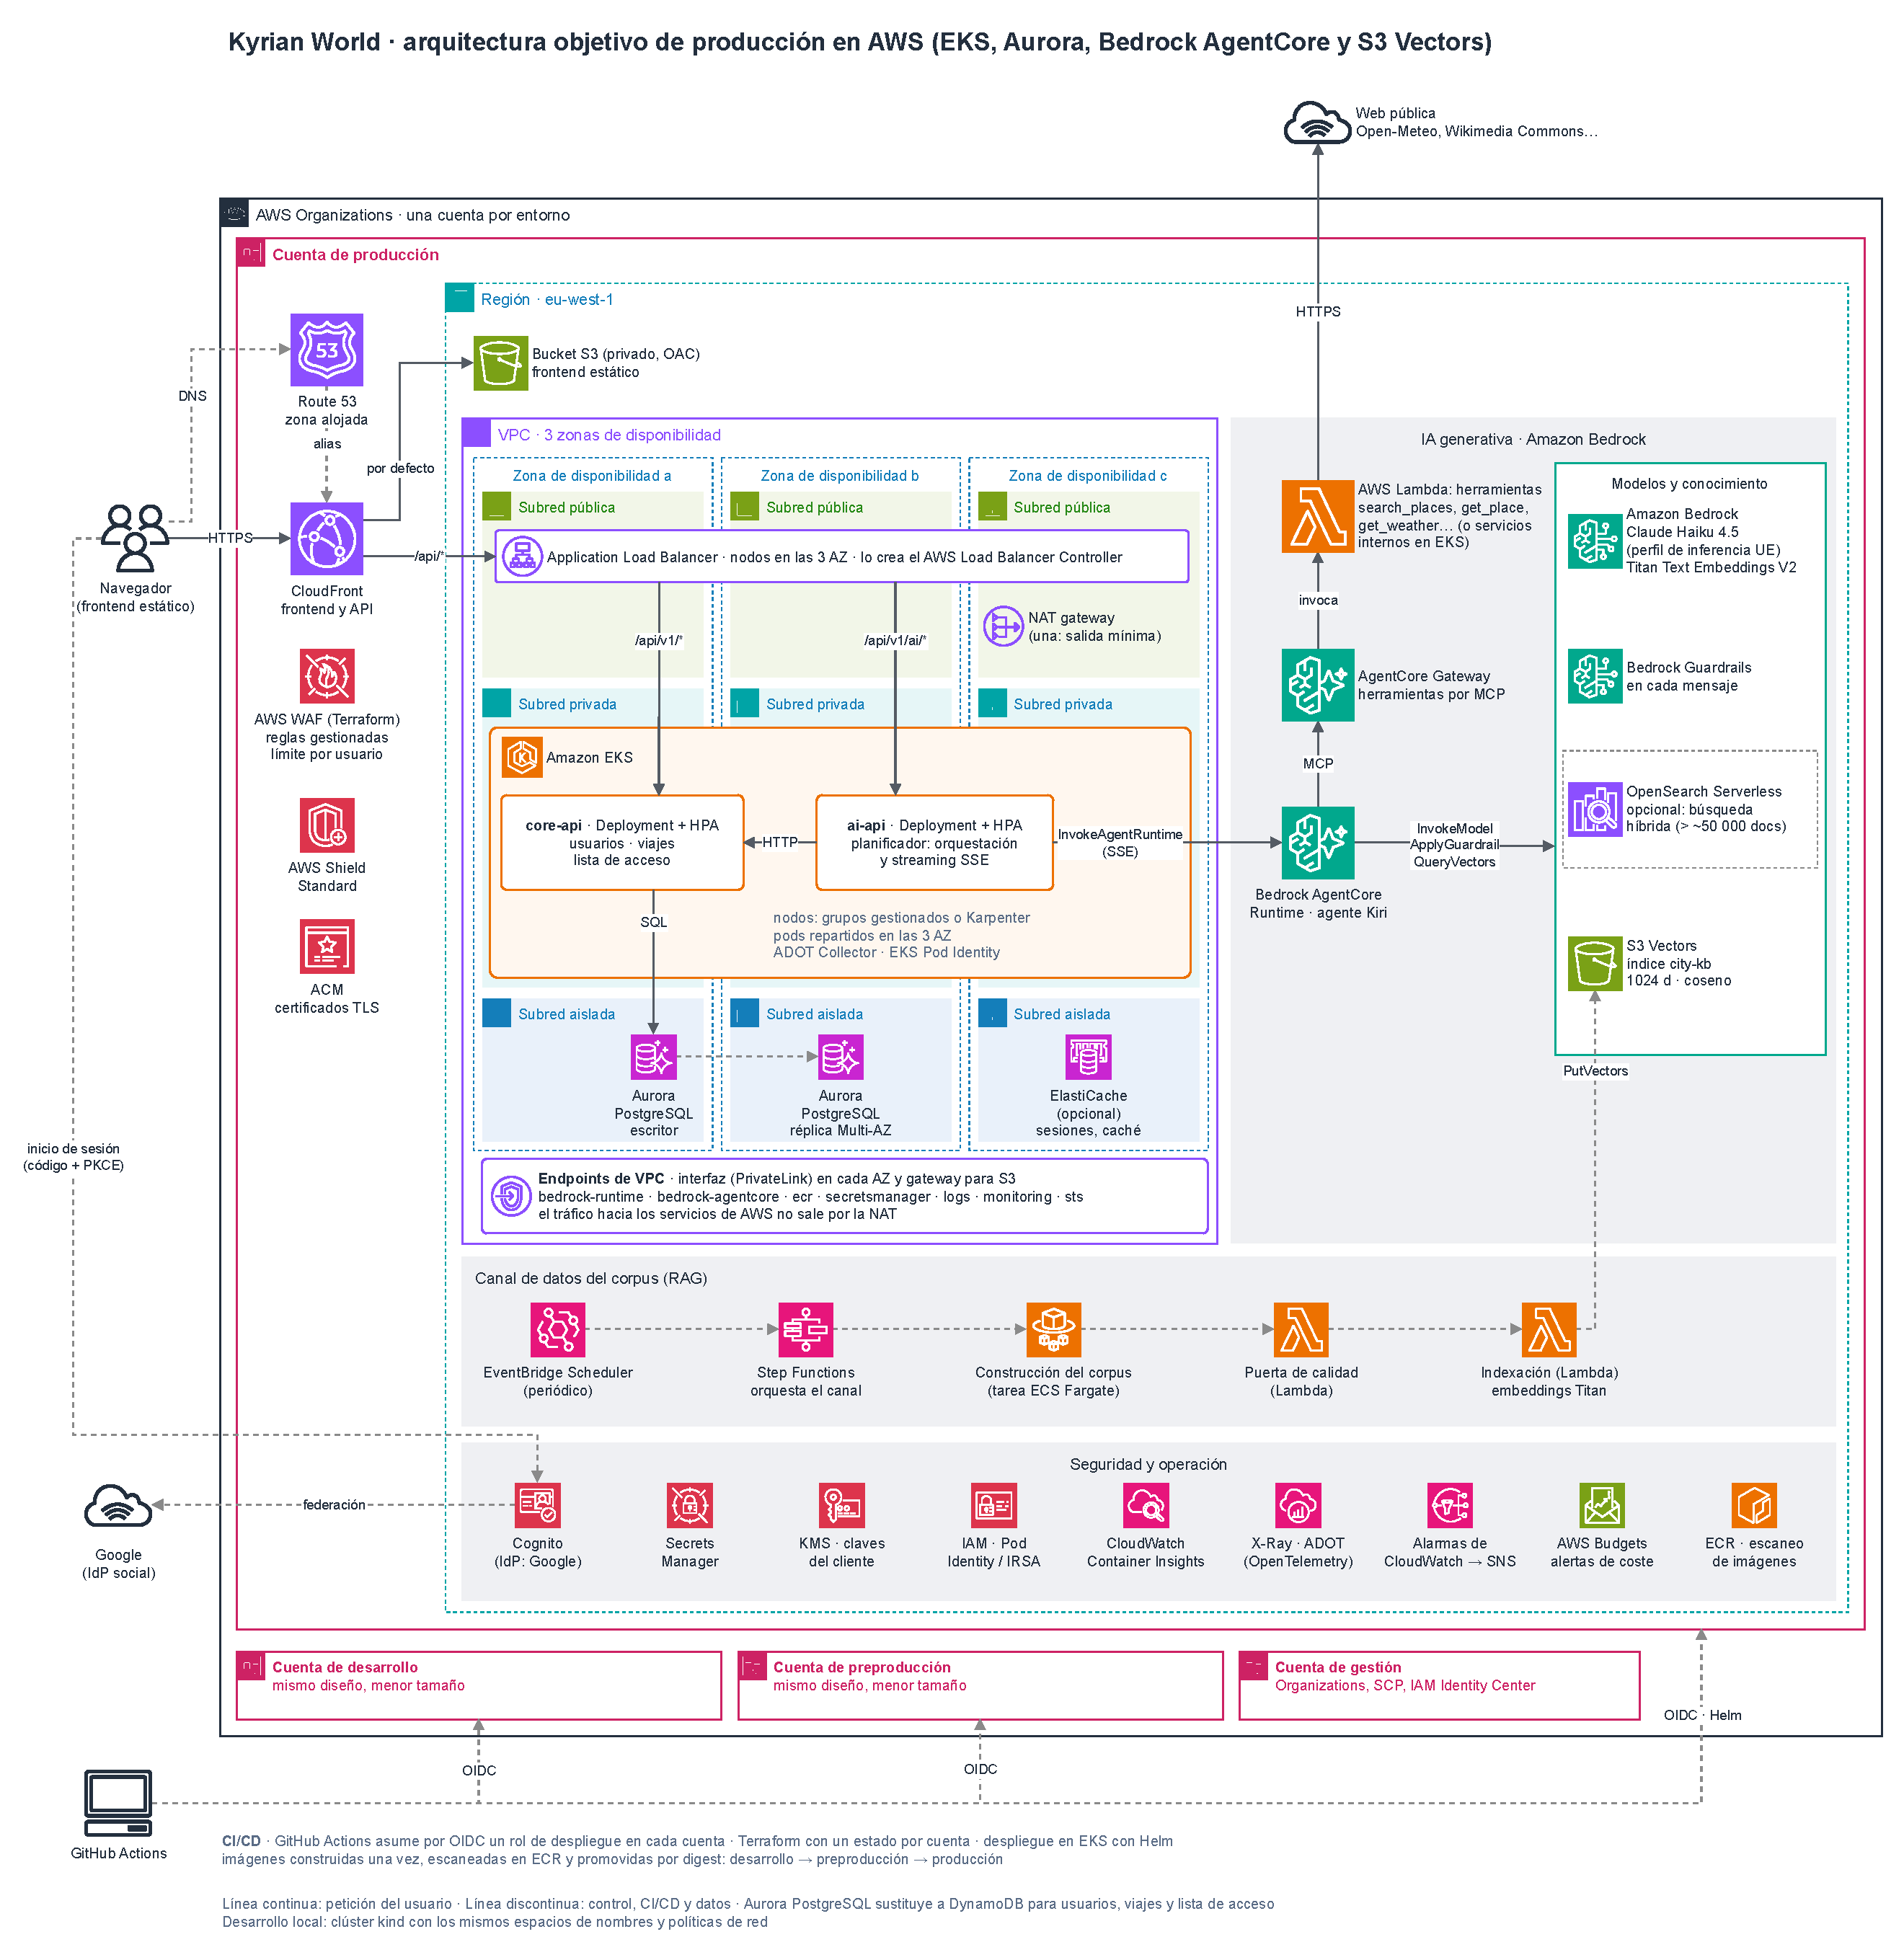
\includegraphics[width=\textwidth]{figs/aws-objetivo.pdf}
\caption{Arquitectura objetivo en AWS para la explotación comercial: tres cuentas (desarrollo, preproducción y producción), servicios en EKS (Kubernetes gestionado) dentro de subredes privadas, Aurora PostgreSQL (base de datos relacional gestionada), agente alojado en Bedrock AgentCore (entorno gestionado para agentes) con sus herramientas expuestas por MCP, búsqueda híbrida opcional con OpenSearch Serverless y observabilidad completa.}\label{fig:objetivo}
\end{figure*}

\subsubsection{Seguridad} La sesión se inicia con Google a través de Cognito (flujo de código de autorización con PKCE,
\emph{Proof Key for Code Exchange}); API
Gateway valida el token y ambos servicios lo vuelven a verificar de forma local contra las claves
públicas, que Terraform inyecta. \code{ai\_api} consulta la lista de acceso de \code{core\_api}
reenviando el token del propio usuario, sin secretos compartidos entre servicios. Cada función tiene
un rol de IAM (gestión de identidades y accesos) con permisos mínimos: sin \code{Scan} en DynamoDB,
solo lectura sobre la base vectorial y Bedrock limitado al perfil europeo del modelo de chat, al de
\emph{embeddings} y a Bedrock Guardrails. No existen claves de acceso de larga duración: en local se
entra con inicio de sesión único (SSO) y la CI usa federación OpenID Connect (OIDC).

\subsubsection{Privacidad, licencias y regulación} Las trazas guardan el identificador opaco del
usuario, nunca su correo; los textos que registran se recortan a 8\,kB y caducan a los 90 días; los registros de acceso
no contienen identidad y los eventos de negocio se seudonimizan con un \emph{hash}. La inferencia
usa el perfil europeo de Bedrock, de modo que los datos se procesan en regiones de la UE (RGPD).
Cada tarjeta muestra su fuente, su enlace y su licencia (CC BY-SA, ODbL), y las fotos libres
llevan su autor; las fotos de alojamientos sin imagen libre se enlazan desde la web del propio
hotel con su crédito, sin copiarlas. Respecto al Reglamento europeo de IA, un asistente
conversacional de este tipo no es de alto riesgo; su obligación es de transparencia (art.~50:
informar de que se conversa con una IA, aplicable desde agosto de 2026), y el diseño va más allá
mostrando de dónde sale cada recomendación.

\subsection{Arquitectura objetivo para producción}\label{sec:prod}

La arquitectura actual está optimizada para la fase en la que está el producto: tráfico de
demostración, disponibilidad permanente y coste mínimo. Si \kyrian{} pasara a explotación
comercial, con tráfico sostenido y clientes B2B, las prioridades cambiarían: latencia estable en
cada turno, aislamiento de red, datos relacionales para informes y facturación, y entornos
separados para probar antes de publicar. La Fig.~\ref{fig:objetivo} muestra la arquitectura
propuesta para esa fase y la Tabla~\ref{tab:objetivo} resume qué cambia y por qué.

\begin{table}[t]
\centering\scriptsize
\caption{De la arquitectura actual a la objetivo.}\label{tab:objetivo}
\begin{tabularx}{\columnwidth}{@{}L{1.55cm}L{1.95cm}Y@{}}
\toprule
\textbf{Actual} & \textbf{Objetivo} & \textbf{Motivo} \\
\midrule
Lambda + Web Adapter & EKS (pods de \code{core-api} y \code{ai-api}) tras un ALB & Sin arranques en frío (hoy, el 10,7\,\% de las invocaciones de \code{ai\_api}), sin el salto del adaptador, escalado por réplicas y despliegues graduales \\
Sin VPC & VPC en 3 zonas: subredes públicas (ALB) y privadas (EKS, datos) & Servicios y base de datos sin exposición pública; \emph{endpoints} privados hacia Bedrock, S3 y ECR \\
DynamoDB & Aurora PostgreSQL multizona & Modelo relacional para usuarios, viajes, accesos e informes; transacciones y consultas \emph{ad hoc} \\
Agente en el contenedor & Bedrock AgentCore Runtime + Gateway (MCP) & Agente gestionado con sesiones aisladas; herramientas extraídas como Lambdas o servicios internos, reutilizables desde otros canales \\
Una cuenta & Organizations: desarrollo, preproducción y producción & Probar cada cambio en un entorno idéntico antes de publicarlo \\
Variables de entorno & Secrets Manager + KMS & Rotación de secretos y claves propias \\
Cuadros de mando & Alarmas, SNS, Budgets, X-Ray/OpenTelemetry & Avisar en lugar de vigilar; trazas distribuidas entre servicios \\
Indexación manual & EventBridge + Step Functions & Corpus reconstruido, validado e indexado de forma programada \\
\bottomrule
\end{tabularx}
\end{table}

\textbf{Qué se conserva.} El borde (CloudFront, WAF y el sitio estático en S3), Cognito, los
modelos de Bedrock y Bedrock Guardrails, la base vectorial y la CI/CD con credenciales temporales
siguen igual. La migración del cómputo es directa porque los dos servicios ya se publican como
imágenes de contenedor y su arquitectura hexagonal aísla la persistencia y el proveedor de modelos
detrás de puertos: pasar a Aurora es escribir un adaptador nuevo, no reescribir los casos de uso.

\textbf{El agente como servicio gestionado.} El servicio de IA en EKS mantiene el contrato de
eventos SSE con el navegador y delega el bucle del agente en Bedrock AgentCore Runtime, que admite
respuestas en \emph{streaming}. Las herramientas salen del contenedor y se publican a través de
AgentCore Gateway como servidor MCP: las de consulta (búsqueda, ficha, clima) como funciones
Lambda y las que escriben en el itinerario como servicios internos del clúster. Así se pueden
escalar, versionar y auditar por separado, y otros canales (por ejemplo, una aplicación dentro de
un asistente generalista) pueden reutilizarlas.

\textbf{Entornos y desarrollo local.} Cada entorno vive en su propia cuenta con la misma
definición de Terraform, y las imágenes se promueven de uno a otro por su \emph{digest}, de modo
que lo que se prueba en preproducción es exactamente lo que llega a producción. En local, un
clúster kind reproduce los mismos espacios de nombres, políticas de red y cuentas de servicio,
con PostgreSQL en un contenedor, de forma que la segregación que se valida en el portátil es la
misma que la del despliegue.

\begin{table}[t]
\centering\scriptsize
\caption{Coste fijo orientativo del entorno de producción objetivo (precios de lista, eu-west-1; preproducción y desarrollo usan versiones más pequeñas).}\label{tab:prodcoste}
\begin{tabularx}{\columnwidth}{@{}Yr@{}}
\toprule
\textbf{Componente} & \textbf{\$/mes} \\
\midrule
Plano de control de EKS & $\approx$75 \\
Nodos (3 instancias medianas, una por zona) & $\approx$190 \\
Aurora PostgreSQL (escritor + réplica) & $\approx$130 \\
Puertas NAT y \emph{endpoints} privados & $\approx$120 \\
Balanceador de aplicaciones & $\approx$25 \\
WAF, alarmas, Secrets Manager y trazas & $\approx$20 \\
\midrule
\textbf{Total fijo (solo producción)} & \textbf{$\approx$560} \\
Bedrock, AgentCore y base vectorial & por uso \\
\bottomrule
\end{tabularx}
\end{table}

Pasar de unos pocos dólares a unos 560\,\$ al mes de coste fijo es el precio de la latencia
estable, el aislamiento y los entornos separados (Tabla~\ref{tab:prodcoste}). Por eso la
arquitectura actual es la adecuada mientras el tráfico sea de demostración, y la objetivo se
justifica a partir de dos clientes B2B: una sola licencia de 400\,€/mes ya cubre unas tres cuartas
partes de ese coste fijo. La arquitectura actual cumple así O4: siempre en línea, multizona y sin
coste fijo relevante, con un camino de crecimiento ya diseñado.
